\section{První testování - během vývoje s odbornou osobou}

První uživatelské testování výsledné aplikace proběhlo při jejím vývoji - 19. 9. 2019. V době testu byly připravené základní možnosti vkládání a úprav většiny entit v systému (skladové položky, dodavatelé atp.) a necelé čtyři ze stěžejních úloh - příjem dodávky, naskladnění, inventura a část přesunu zboží.\\
Aplikaci testovala osoba, která má zkušenosti se starým skladovým systémem Sysel v roli vedoucího skladu.\\
Testování proběhlo při neformálním setkání v běžné kanceláři, testera jsem instruoval k tomu, aby použil svůj notebook pro zobrazení režimu správce skladu a mobilní telefon pro roli skladníka. Zatímco na počítači bylo vše v pořádku, neboť byl použit Google Chrome, ve kterém aplikaci spouštím i při vývoji, na mobilním zařízení nejprve nastal malý problém, a to z důvodu použití prohlížeče \emph{Samsung Internet}, který nepodporuje některé moderní javascriptové konstrukce, na které aplikace spoléhá. Ačkoliv toto nebude pro samotné použití aplikace problém, protože cílové zařízení pro skladníky je jasně dané a aplikace se tam bude otvírat ve WebView, i přesto není na škodu zachovat kompatibilitu i s jinými mobilními prohlížeči, třeba i pro potřeby vedoucích, aby taktéž mohli pracovat z mobilních zařízení. Již před testováním jsem věděl, že je potřeba zavést nějakou detekci prohlížečů a případně uživatele informovat o nekompatibilitě aplikace se zvoleným browserem, ale po této skutečnosti jsem ještě zvýšil této úpravě prioritu.\\
Výstupem z tohoto testování vývojové verze aplikace je seznam postřehů, chyb a návrhů na zlepšení, které jsou k nalezení v příloze \ref{ap:testing_notes}.\\
Zde je vhodné poznamenat, že zhruba pětinu všech požadavků a chyb jsem již nějakým způsobem evidoval i před testováním - buďto formou \emph{\uv{TODO} komentářů} přímo v kódu aplikace, nebo kartami v Trellu, avšak pro kompletnost zápisu jsem je ponechal i tam.

%%%%%%%%%%%%%%%%%%%%%%%%%%%%%%%%%%%%%%%%%%%%%%%%%%%%%%%%%%%%%%%%%%%%%%%%%%%%%%%%
%%%%%%%%%%%%%%%%%%%%%%%%%%%%%%%%%%%%%%%%%%%%%%%%%%%%%%%%%%%%%%%%%%%%%%%%%%%%%%%%
%%%%%%%%%%%%%%%%%%%%%%%%%%%%%%%%%%%%%%%%%%%%%%%%%%%%%%%%%%%%%%%%%%%%%%%%%%%%%%%%
%%%%%%%%%%%%%%%%%%%%%%%%%%%%%%%%%%%%%%%%%%%%%%%%%%%%%%%%%%%%%%%%%%%%%%%%%%%%%%%%

\section{Druhé testování - alfa verze kompletní aplikace}\label{sec:usertest}

Dne 6. 12. 2019 proběhlo druhé uživatelské rozhraní, které bylo na rozdíl od prvního testování mnohem obsáhlejší. Vydal jsem se do dvou skladů menších rozměrů, ve kterých jsem otestoval celkem čtyři osoby zde pracující.\\
Průběh testování probíhal s každou testovanou osobou stejně, podle následujícího rozpisu:
\begin{enumerate}
	\item Pokud byl ve skladu používán již nějaký skladový systém, pozoroval jsem chvíli, jak se s ním pracuje a jaké jsou nejdůležitější úkony.
	\item Položil jsem testované osobě několik otázek dle \emph{Dotazníku před testováním} (viz příloha \ref{ap:testing_questions}).
	\item Provedli jsme samotné testování aplikace, dle připravených úkolů (viz příloha \ref{ap:testing_tasks}).
	\item Položil jsem testované osobě několik dalších otázek, dle \emph{Dotazníku po testování} (viz příloha) \ref{ap:testing_questions}).
	\item Jako poděkování jsem nabídl vánoční perníčky.
\end{enumerate}

V tomto textu budu vypisovat pouze nejdůležitější odpovědi a poznatky z testování, zápis požadavků a problémů zpracovaný do strukturovaného seznamu je dostupný v příloze \ref{ap:testing_requirements}. Také nebudu zmiňovat celá jména testovaných osob, neboť to pro výstup testu není podstatné.
\\
Během samotného testování aplikace jsme používali reálná zařízení Zebra TC-25, na kterém jsem měl předinstalovanou aplikaci s podporou čtečky čárových kódů. Také jsem měl vytištěných několik čárových kódů, kterými se identifikují umístění ve skladu a dále několik kódů reprezentující skladové položky. Kromě Zebry - na které jsem testoval především roli \emph{skladníka}, jsme vždy využili i notebook, který je běžně ve skladu používán - na tom se naopak testovala role \emph{vedoucího skladu}.

%%%%%%%%%%%%%%%%%%%%%%%%%%%%%%%%%%%%%%%%%%%%%%%%%%%%%%%%%%%%%%%%%%%%%%%%%%%%%%%%
%%%%%%%%%%%%%%%%%%%%%%%%%%%%%%%%%%%%%%%%%%%%%%%%%%%%%%%%%%%%%%%%%%%%%%%%%%%%%%%%

\subsection{Testování v prvním skladu}

Nejprve jsem začal ve skladu e-shopu, jehož sortimentem je převážně obuv, přípravky pro péči o tělo a zdraví, výbava domácnosti a také elektronika. Sklad se nachází v samostatné místnosti v průmyslové budově a obsahuje odhadem kolem čtyř set umístění, přičemž \uv{umístění} je krabice polepená štítkem, kterých je na sobě mezi čtyřmi až šesti, a jsou vyskládány v řadách.\\
V tomto skladu je aktuálně používán skladový systém Sysel, ze kterého vycházela i analýza požadavků pro nově tvořený systém, takže se nabízela možnost přímého srovnání obou systémů.\\
Ještě před započetím testování jsem si zavedl do nového systému dvě reálná umístění tohoto skladu a jeden konkrétní výrobek. Bohužel kvůli povaze skladovaného zboží jsem nenašel více stejných skladových položek, a tak jsme nemohli efektivně simulovat práci s více kusy stejné položky.

%%%%%%%%%%%%%%%%%%%%%%%%%%%%%%%%%%%%%%%%%%%%%%%%%%%%%%%%%%%%%%%%%%%%%%%%%%%%%%%%

\subsubsection{Postřehy z testování s první osobou}
\emph{Žena, 42 let, dříve zdravotní sestra, nyní majitelka e-shopu.}

\paragraph{Dotazník před testováním.} Z dotazníku provedeného před samotným testováním vyplynulo, že první testovaná osoba od skladového systému nejvíce očekává informace o umístění požadovaného kusu zboží během vyskladňování. Dále jí vyhovují režimy pípání při načítání kódů - krátké pípnutí jako potvrzení a dlouhé jako chyba. Také považuje za důležité mít v systému funkci průchodu historie umístění položky - pro případ, že na deklarovaném umístění se položka ve skutečnosti nenachází. Naopak jako problematické označila například nutnost posouvat se na obrazovce až na konec v případě, že něco naskladňuje, protože nejnovější položka se přidá na konec seznamu. Také jí vadí absence evidence kapacity umístění, kterou si vede v separátním souboru uloženém na notebooku, který je ve skladu.\\

\paragraph{Testování nové aplikace.} Co se týká testování nového systému, přistupovala k němu spíše s rozvahou, často tápala, kudy má pokračovat, nebo co má zadávat. Toto bylo částečně způsobeno tím, že na rozdíl od Sysla je v novém systému prohozeno pořadí \uv{napípávání} kusu zboží a umístění, ze kterého je sebráno, či na které je uloženo. Největší problémy dělalo hledání přidávání nových věcí - ať už skladových položek nebo úkolů, které je řešeno pluskem ukotveném v pravém dolním rohu obrazovky. Během testování mi bohužel příliš nesdělovala své myšlenky, které by byly přínosné pro případné úpravy, největších problémů jsem si ale i přesto všiml a poznamenal jsem si je.\\
Některé úkony prováděla poprvé, neboť je nedělá ani v současném skladovém systému - jednalo se například o založení nové skladové položky. Po nalezení příslušné akce bez problémů vyplnila potřebná pole, bohužel ale nedokázala určit, která pole jsou povinná\footnote{Povinnost polí je ve formulářích označována hvězdičkou a při chybě jsou pole označena červeně, viz obrázek \ref{picture:test:required_fields}. Toto označení považuji i po tomto testu za dostatečné.}.\\

\begin{figure}[h]

\includegraphics[width=\textwidth]{../png/app_testing/required_fields.png}
\caption[Označení povinných polí formuláře]{Označení povinných polí formuláře: Název je povinný a uživatel v něm již měl kurzor, nebo se pokusil formulář odeslat. Model je povinný, ale uživatel do něj ještě neklikl. Výrobce je výběr ze seznamu, ale povinný není.} \label{picture:test:required_fields}
\end{figure}

Častokrát jsme také narazili na to, že některé úkony jsou v novém systému složitější, než ve starém - již například zmiňovaná nutnost nejprve \uv{napípnout} umístění. Starý systém nabízel automatické doplnění umístění, pokud byl \uv{napípnut} výrobek, který je v systému pouze na jednom místě. Tato funkce ale někdy nebyla stoprocentně spolehlivá, a tak jsem se rozhodl mechanismus předělat tak, aby se vždy nejprve volilo umístění, od čehož jsem si sliboval snížení chybovosti především ve větších skladech. Rozumím ale argumentu, že pro sklad, který víceméně celý spravuje jeden člověk, je toto zbytečné ztížení, avšak již v době psaní této práce je vypsáno nové téma, které bude na tuto práci navazovat a jehož cílem bude právě optimalizace procesů na malých skladech - považuji tedy za korektní svůj současný přístup, a to, že v systému lze provést vše, kvalitně, avšak někdy zbytečně zdlouhavě, a efektivnější procesy se mohou dále optimalizovat.

\paragraph{Dotazník po testování.} Po skončení testování jsem se vyptal na několik věcí přímo se týkajících nového systému. Jako největší slabinu označila především menší písmo a pro ni nižší přehlednost, na druhé straně uvítala zobrazování fotografií skladové položky. Nejvíce jí chyběla možnost zadat přímo počet kusů položky, \uv{napípávání} všech jednotlivých kusů postupně jí nevyhovovalo. Na otázku, zda by jí dávalo smysl namísto pípání, nebo jako doplněk k němu, používat vibrace zařízení, reagovala, že jí to připadá jako zbytečnost, protože zvukový signál prý vnímá lépe.

%%%%%%%%%%%%%%%%%%%%%%%%%%%%%%%%%%%%%%%%%%%%%%%%%%%%%%%%%%%%%%%%%%%%%%%%%%%%%%%%

\subsubsection{Postřehy z testování s druhou osobou}
\emph{Muž, 40 let, dle svých slov \uv{majitel největšího e-shopu v ČR s mizerným skladovým systémem}\footnote{První část tvrzení není pravda, druhou nemohu objektivně posoudit.}.}

\paragraph{Dotazník před testováním.} Již z dotazníku provedeného před testování bylo zřejmé, že se jedná o člověka, který se se skladovými systémy již setkal, a to i ve větším měřítku než pouze ve skladu e-shopu. Co se konkrétně aktuálně používaného systému - tedy Sysla - týká, vyhovuje mu především propojení s e-shopem, rychlost a individuální řešení. Na druhé straně si ale stěžuje na některé kostrbaté funkce, jako příklad uvedl, že když přiřadí EAN k nové položce, ale ten stejný EAN už byl dříve použit, tak se ze staré položky odebere, aniž by o tom byl uživatel informován. Od skladového systému očekává především efektivní využití zaměstnanců, jedná-li se o velký sklad, a také snížení chybovosti. Za nejpalčivější procesy současného řešení označil expedici a inventuru.

\paragraph{Testování nové aplikace.} V systému se pohyboval velmi rychle a většina zádrhelů byla způsobena spíše tím, že si chtěl něco upřesnit, nebo mi k tomu dát zpětnou vazbu. Efektivně využíval našeptávací pole, ve kterých začal vždy psát a klávesou enter potvrzoval zvolené položky, na rozdíl od předchozí testované osoby, která více používala myš. S přidáváním nových věcí pomocí šipky či pluska v pravém dolním rohu problém neměl, pouze na domovské obrazovce, kde se tento prvek používá pro tvorbu nových úkolů, mu přijdou dva kliky zbytečné a radši by měl seznam dostupný přímo, aby úkoly tvořil jen jedním kliknutím. Při naskladňování byl lehce zmatený nutností pípat nejprve umístění a teprve poté skladové položky, ale rychle se nový postup naučil. Při otázce, jak ze systému zjistí, kde požadovanou položku nalezne, poměrně překvapivě šel hledat do zadání, přestože tato informace se vztahuje ke konkrétní položce. Až když v zadání tuto informaci nenašel, zkusil rozkliknout skladovou položku, kde už požadovaná informace byla. Během testování zanadával pouze jedenkrát, a to ve chvíli, kdy zjistil, že při přesunu položek mezi umístěními musí nejprve všechny položky \uv{napípat} při jejich zvednutí, a znovu při jejich položení na cílové umístění. Tento proces mi přišel od stolu poměrně logický, protože pouze tak je možné zaručit, že skladník položí opravdu všechny položky, ale uživatel to vidí jinak - tento konkrétní tester při tomto zjištění aplikaci pojmenoval \uv{skladový systém buzerant}.

\paragraph{Dotazník po testování.} Po testování jsem se jako v prvním případě zeptal na několik dopřesňujících otázek. Na novém systému oceňoval nový a moderní design, přišlo mu ale že většina důležitých informací je vždy orientována až moc do levé horní části stránky. Uvítal novou možnost nastavit jednomu účtu role skladníka i vedoucího současně, u práce se skladovými položkami mu ale chyběla možnost přímo nastavit jejich množství. Co se konfigurovatelnosti domovské obrazovky týká, navrhuje i možnost zobrazovat úkoly ne ve sloupcích, ale v řádcích. Také má zkušenosti se skladováním zboží více různých majitelů, naopak šarže mu blízké nejsou, ale rád by o nich zjistil více, protože jimi označené zboží plánuje do budoucna také skladovat.

%%%%%%%%%%%%%%%%%%%%%%%%%%%%%%%%%%%%%%%%%%%%%%%%%%%%%%%%%%%%%%%%%%%%%%%%%%%%%%%%
%%%%%%%%%%%%%%%%%%%%%%%%%%%%%%%%%%%%%%%%%%%%%%%%%%%%%%%%%%%%%%%%%%%%%%%%%%%%%%%%

\subsection{Testování v druhém skladu}

Po otestování prvních dvou osob jsem se přesunul do druhého skladu, který na rozdíl od toho prvního žádný skladový systém nepoužívá, přestože počet skladovaných produktů také není nejmenší. Osoby pracující v tomto skladu si ale veškerá umístění pamatují, a umístění by zde ani nebylo zcela jednoduché zřídit, neboť se jedná víceméně o chodbu a jednu místnost v přízemí rodinného domu, kde je na první pohled vše uloženo tam, kam se to zrovna vešlo. Jelikož se ale i přesto o zavedení skladového systému do budoucna uvažuje - pravděpodobně již v nových prostorech, kam by se měl sklad přemístit, bylo testování na místě.\\
Kvůli nižším teplotám v samotném skladu jsme testování prováděli v zázemí, u notebooku, a umístění jsme simulovali mými čárovými kódy, které jsem měl předem vytištěné. Jako skladové položky jsme poté využili běžné zboží, které bylo dostupné v kuchyni, a od kterého jsme měli k dispozici více než jeden kus.

%%%%%%%%%%%%%%%%%%%%%%%%%%%%%%%%%%%%%%%%%%%%%%%%%%%%%%%%%%%%%%%%%%%%%%%%%%%%%%%%

\subsubsection{Postřehy z testování s třetí osobou}
\emph{Žena, 30 let, živnostnice, skladník na expedici}

\paragraph{Dotazník před testováním.} Zkušenost se skladovými systémy zde byla nulová, čímž odpadla i většina dalších otázek, které jsem v dotazníku před testováním pokládal. Co se požadavků na takový systém týká, očekávala by především časové usnadnění práce ve smyslu zlepšení orientace, případně i poskytování vhodných statistik jako například trendů ve vyskladňování zboží - doporučování k objednání apod. Během této diskuze jsme se dostali až k bodům, které se již týkají spíše systému e-shopu, jako například nabízení slev na produkty, které se dlouhodobě neprodávají, ale přesto jsem si je poznamenal.

\paragraph{Testování nové aplikace.} Během samotného testování projevila poměrně velkou komunikativnost, sdílela své pocity a myšlenkové pochody, což bylo pro účely uživatelského testování naprosto skvělé. Z jejího testování tedy mám nejdelší zápis a nejvíce návrhů na zlepšení, o kterých budu dále přemýšlet. Stejně jako se již objevilo dříve, měla poměrně problém s pluskem v pravém dolním rohu, avšak jakmile jej jednou nalezla, tak již věděla, co v něm očekávat a práce se rapidně zrychlila. Mezi nejzajímavější návrhy ke zlepšení patří možnost zasílat skladníkům přímé notifikace, že jim byl přiřazen nový úkol. Poměrně problematické pro ni bylo pochopit, že nejprve je vždy nutné naskenovat kód umístění a teprve poté kód skladové položky - i když již tento proces procházela poněkolikáté, tak skoro vždy provedla skenování v opačném pořadí, přestože systém poskytuje hlášky, jaké skenování je očekáváno. Z toho tedy vyplynulo, že se hlášky musí ještě zlepšit - prostor pro to je a hned při testování jsem si zapsal návrhy na konkrétní úpravy. Podobný problém se zobrazovanými informacemi na stránce nastal i při vyskladňování, ve kterém ji mátla informace o umístění, na které má vyskladňované zboží přemístit - místo toho si myslela, že na uvedeném umístění najde zboží k vyskladnění. I na tento bod jsem měl již při testování zapsaný návrh na zlepšení.\\
Diskuze proběhla také nad funkcí záznamu stráveného času, u kterého marně hledala funkcionalitu pauzy, kterou jsem hodlal do aplikace tak jako tak přidat. Matoucí ale byl dialog při odchodu z rozpracované úlohy, který se ptá, zda chce uživatel uložit čas - v testerce vyvolal dojem, že když čas uloží nyní, tak už nikdy později nepůjde přidat čas další. 

\paragraph{Dotazník po testování.} Odpovědi na otázky výstupního dotazníku byly pozitivní, avšak vzhledem k absenci zkušeností se skladovými systémy bohužel nedokázala říci, zda jí v novém systému něco chybí. Kladně se stavila ke všem návrhům na vylepšení - tj. mít možnost přidání vibrací zařízení, možnost nastavit si seznamy na domovské obrazovce, možnost zadávat počty kusů přímo, bez nutnosti vše pípat a také podporu zkratek v systému pomocí načtení čárového kódu.

%%%%%%%%%%%%%%%%%%%%%%%%%%%%%%%%%%%%%%%%%%%%%%%%%%%%%%%%%%%%%%%%%%%%%%%%%%%%%%%%

\subsubsection{Postřehy z testování s čtvrtou osobou}
\emph{Žena, 32 let, živnostnice, majitelka e-shopu.}

\paragraph{Dotazník před testováním.} Jelikož se jedná o stále stejný sklad, ani poslední testovaná nemá zkušenosti se skladovými systémy, a proto byla většina otázek ze sekce \uv{před testováním} přeskočena. Od skladového systému očekává, že jí řekne, kde se skladová položka nachází, další nápady jsem z ní ale v této části testování nedostal.

\paragraph{Testování nové aplikace.} Při testování aplikace se projevila jako učenlivá, ale dosti skeptická k novým věcem, největší problém bylo vždy požadovanou věc v systému nalézt, ale po jejím prvním projití byl již druhý průchod velmi rychlý. Z tohoto testování také pochází některé citace, které nešlo do textu nezahrnout:
\begin{itemize}
	\item \emph{Během hledání, kudy se zakládá nová skladová karta:} \uv{Tady nikde není nový produkt... Tohle? Sorry jako ale takovýhle plus? ... Ježiš marja zase dole v pravym rohu!}
	\item \emph{Během vyskladňování typu \uv{expedice} (což vlastně znamená přemístění na jiné místo, kde se bude balit):} \uv{Já si to teda vezmu z U2\footnote{označení umístění} a přemístím to na U3 a to je uplně dementní, na tom strávíme hrozně moc času!}
\end{itemize}
Při dotazu, zda nějak naloží s informací, že daná skladová položka je někdy v krabici, která má vlastní kód, a uvnitř je deset kusů zboží, prohlásila, že namísto aby si vytvořila v systému nový kód této položky, který bude reprezentovat 10 kusů, tu krabici rozbalí a po jedné položce naskladní. Na rozdíl od předchozích testerů neměla žádné problémy s pochopením pořadí pípání umístění a položek, v tomto se zorientovala velmi rychle. U dialogu se záznamem stráveného času namítla poměrně věcný bod, že čas by se mohl ukládat vždy, protože takto by pro skladníka bylo jednodušší s časem manipulovat - načež jsem usoudil, že tuto funkcionalitu budu muset ještě znovu promyslet.

\paragraph{Dotazník po testování.} Při pokládání otázek po testování jsem byl opět svědkem odmítavého přístupu k zavedení podobného systému, a to větou \uv{Já bych to nepoužívala ani náhodou, přijde mi to hrozně zdlouhavý, že bych strávila víc času, než prostě jen vezmu, zabalim, nalepim štítek.}. Systém jako takový ale špatně nedopadl, veškeré potřebné informace zobrazoval, dokonce jí přišlo jako dobrý nápad umožnit i vibrace zařízení jako doplněk k pípání, a stejně tak jí dávalo smysl spouštění rychlých akcí za pomoci načtení kódu odkudkoliv z aplikace.

%%%%%%%%%%%%%%%%%%%%%%%%%%%%%%%%%%%%%%%%%%%%%%%%%%%%%%%%%%%%%%%%%%%%%%%%%%%%%%%%
%%%%%%%%%%%%%%%%%%%%%%%%%%%%%%%%%%%%%%%%%%%%%%%%%%%%%%%%%%%%%%%%%%%%%%%%%%%%%%%%

\subsection{Shrnutí testování a největší problémy}

Uživatelské testování jako takové považuji za velmi úspěšné. Aplikace byla použitelná, všechny potřebné věci v ní testeři byli schopni nakonec provést, byť v některých případech k tomu vedla trnitá cesta.\\
Při testování se vyskytlo pouze několik aplikačních chyb, které jsme byli schopni obejít a pokračovat v testu, žádná z chyb nebyla zcela kritická.\\

Jelikož nejpalčivější problémy uživatelského rozhraní se často opakovaly u více testerů, popíšu je nyní hromadně:

\paragraph{Tvorba nových věcí pomocí tlačítka plus v pravém dolním rohu.} Na obrázku \ref{picture:test:add_before} je vidět detail seznamu skladových položek, odkud jsem po testerech chtěl založit novou skladovou položku. Většina z nich měla problém s nalezením žlutého \uv{plus} v pravém dolním rohu, přes které se nová položka přidává. Při příštím použití tohoto tlačítka již vše probíhalo svižně, ale i přesto jsem se rozhodl v reakci na tento problém přidat možnost vkládání položek i na konec tabulky, jak je vidět na obrázku \ref{picture:test:add_after}. Tato volba se zobrazuje pouze na tabletech a větších zařízeních, na mobilních zařízeních je plusko dostatečně v zorném úhlu, a navíc se na zařízeních s Androidem jedná o standardní komponentu, na kterou jsou uživatelé zvyklí.

\begin{figure}[h]
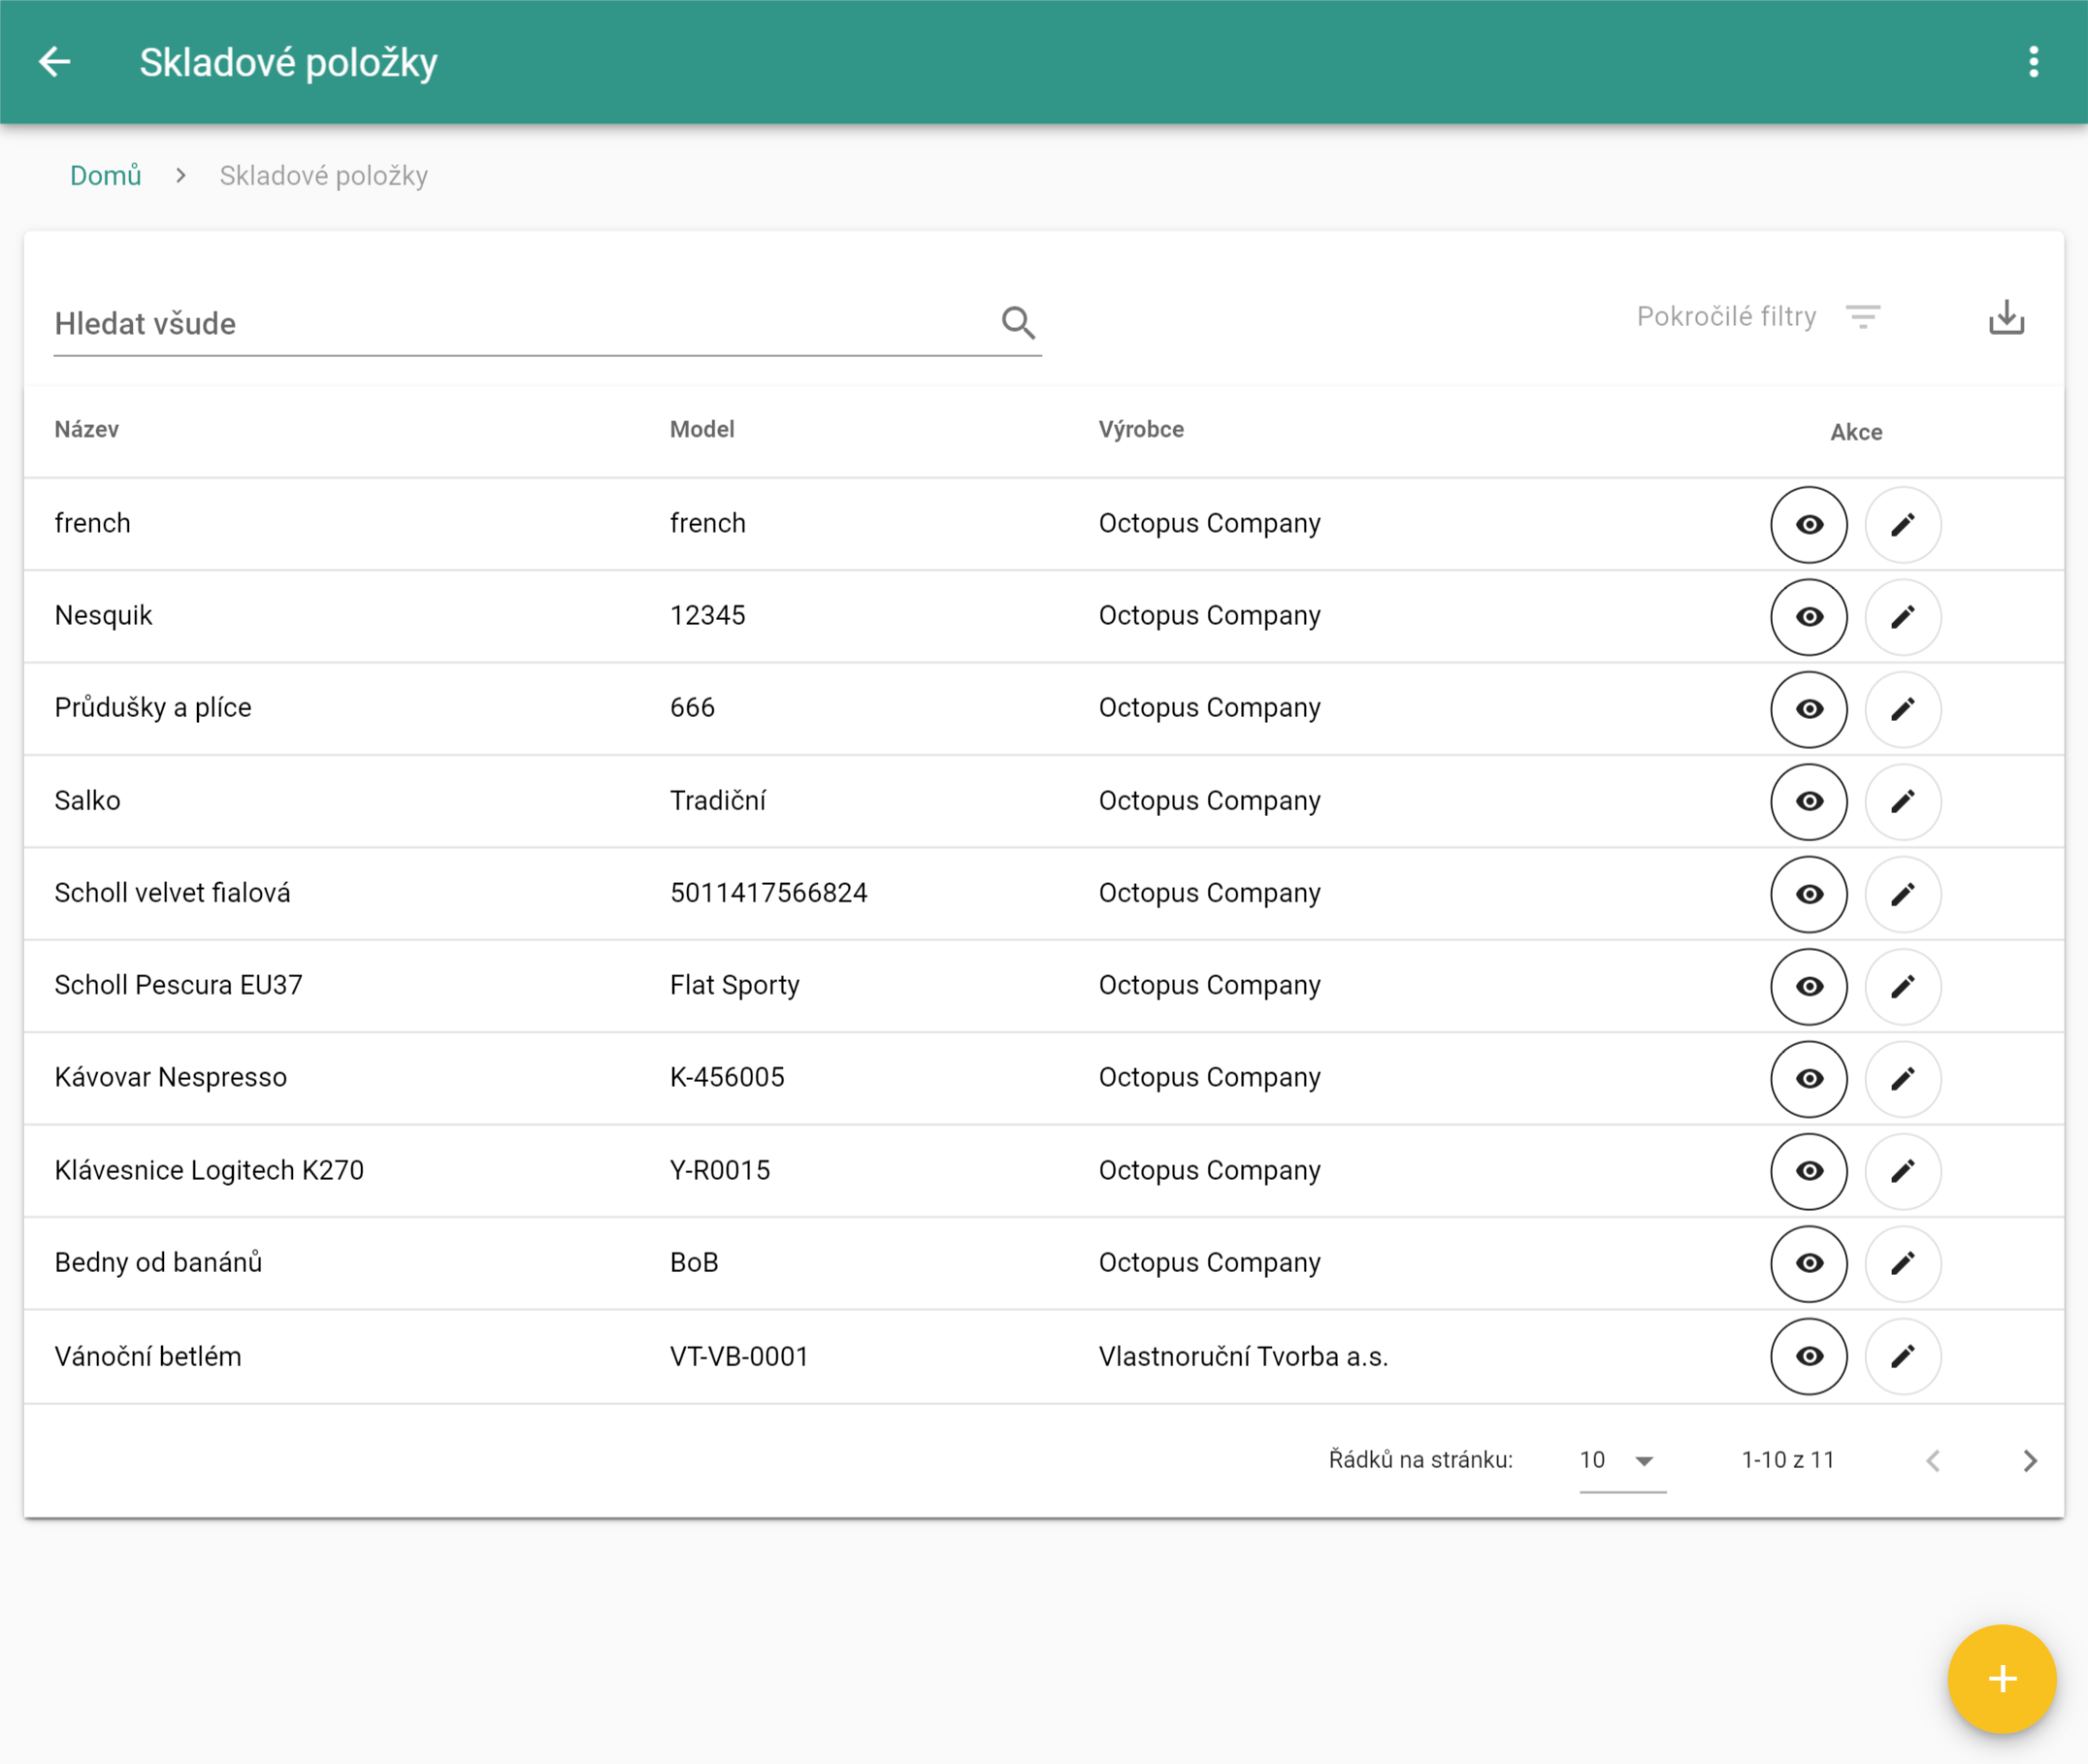
\includegraphics[width=\textwidth]{../png/app_testing/plus_before.png}
\caption{Tvorba nové skladové položky: stav před uživatelským testováním} \label{picture:test:add_before}
\end{figure}

\begin{figure}[h]
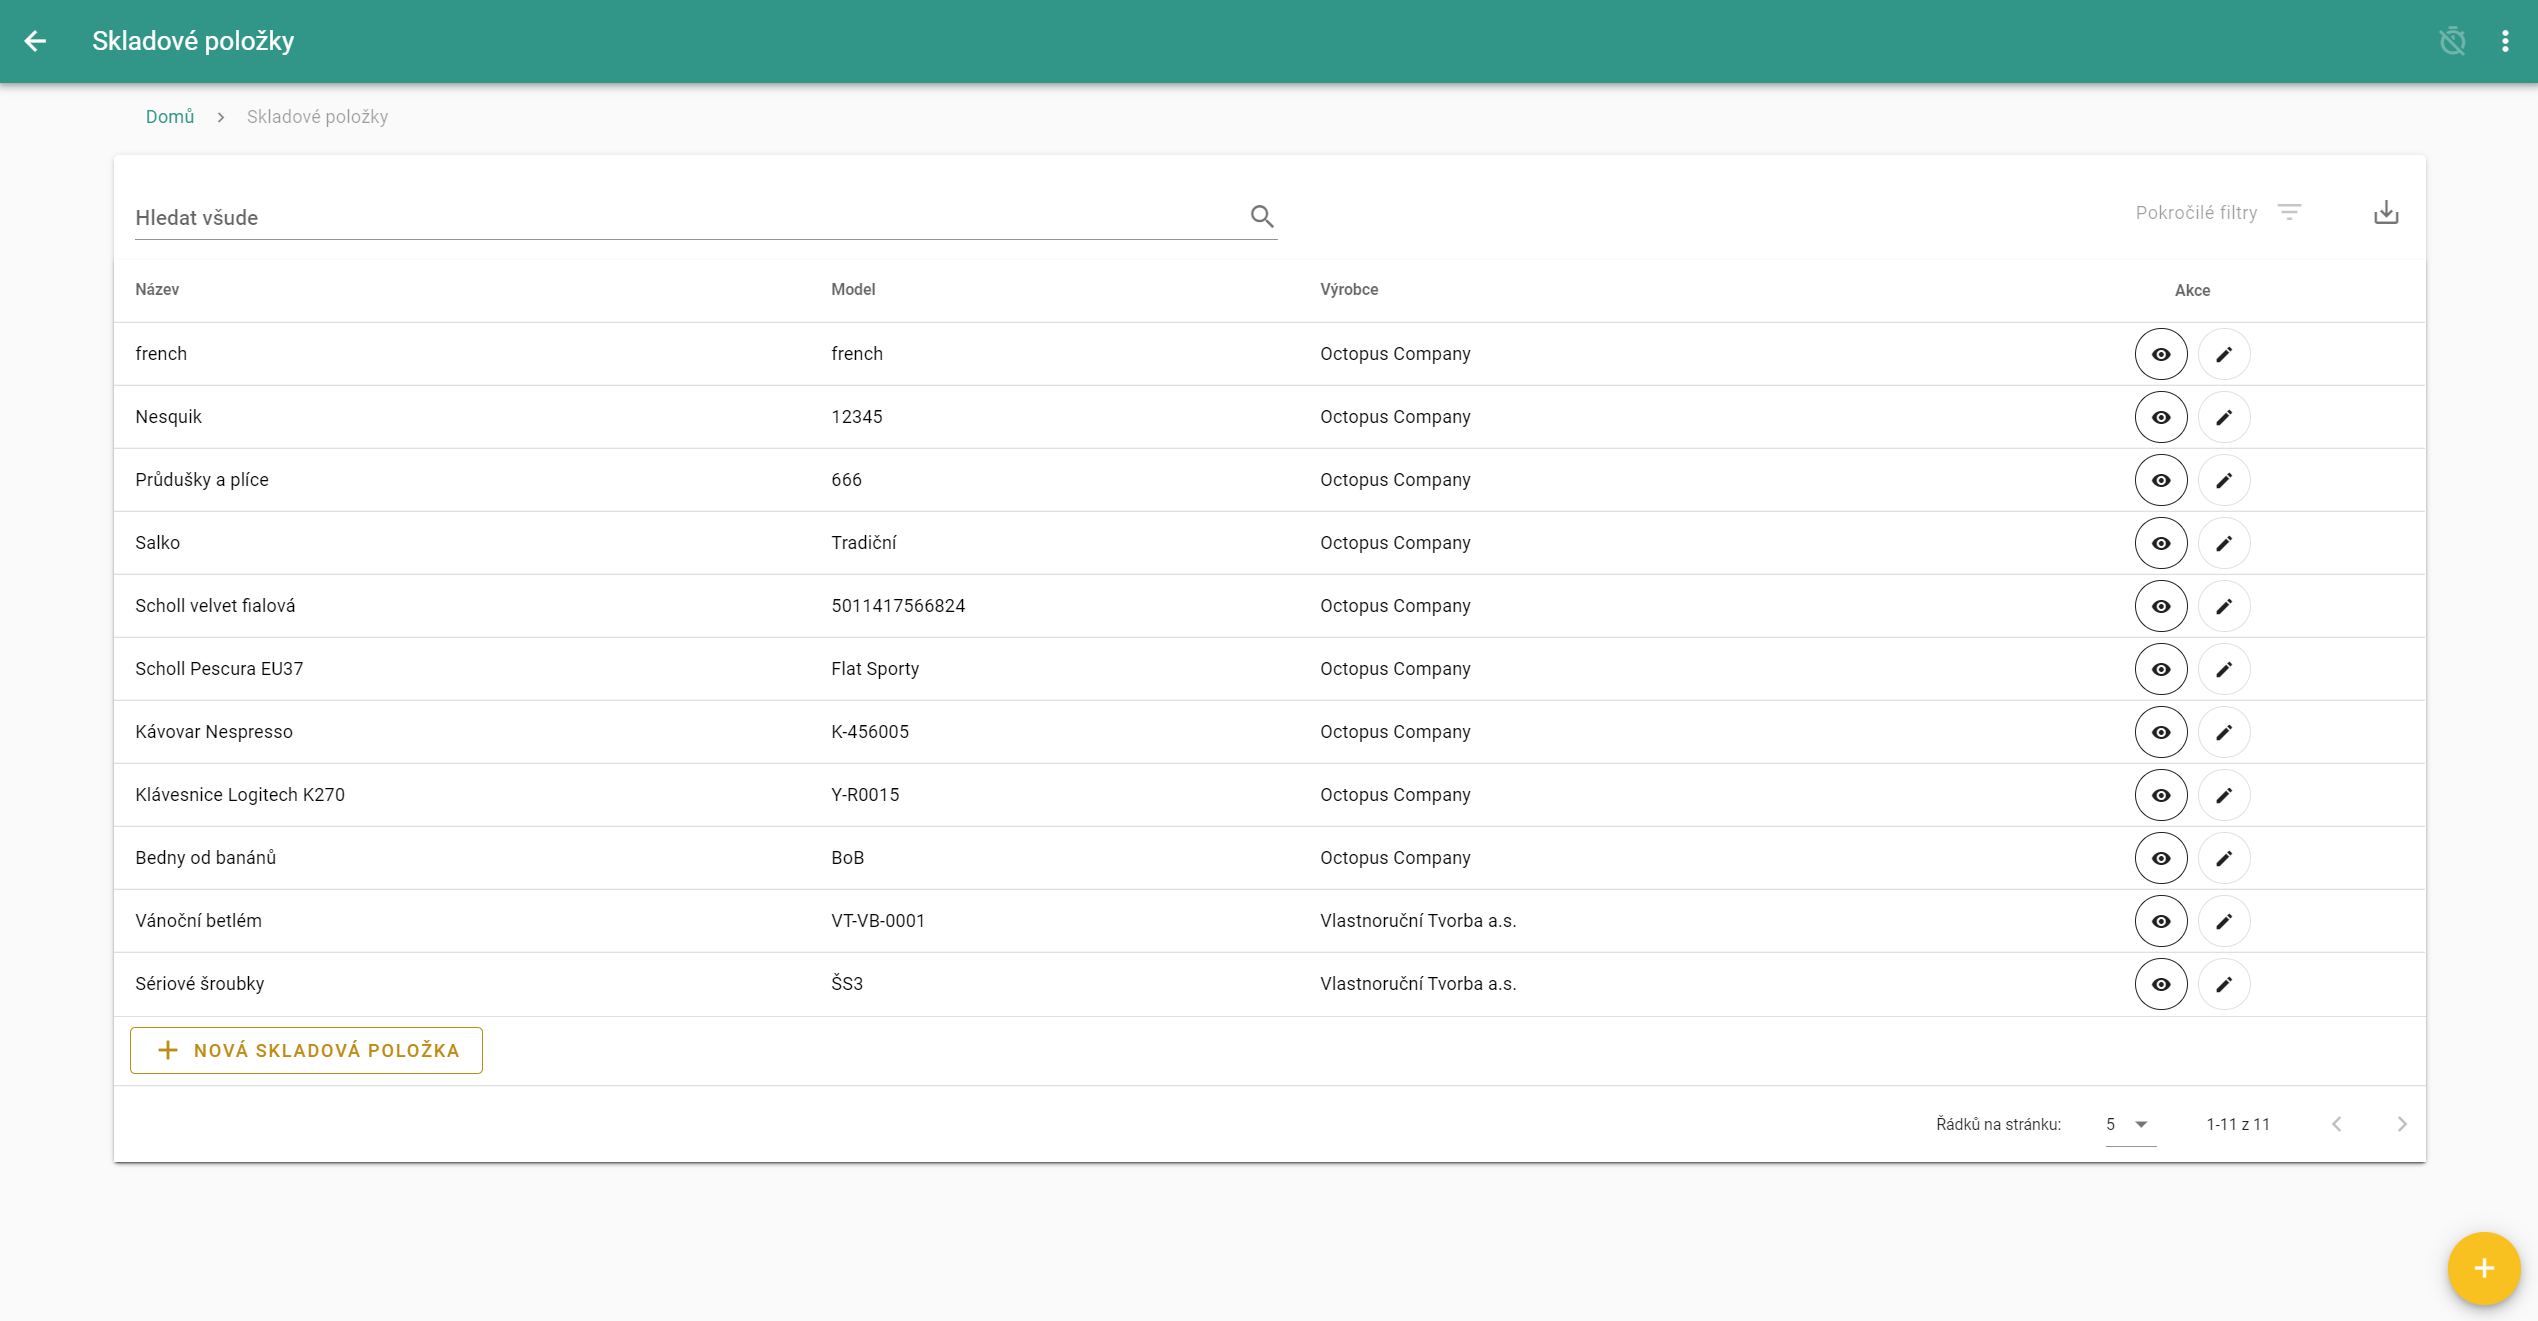
\includegraphics[width=\textwidth]{../png/app_testing/plus_after.png}
\caption{Tvorba nové skladové položky: úprava po testování} \label{picture:test:add_after}
\end{figure}


\paragraph{Přesun mezi umístěními a dvojité pípání položek.} Dalším velmi palčivým problémem, na který si uživatelé stěžovali, byla nutnost znovu zvolit všechny položky, které se chystají přesunout na cílové umístění při přesunu položek, či při vyskladňování typu \uv{expedice}. Při těchto úkolech je potřeba nejprve \uv{napípat} zboží, které skladník \emph{sbírá}, a poté jej \uv{napípat} znovu, při \emph{pokládání} na cílové umístění. Při přesunech, které mají pevně dané cílové umístění může být ale druhé pípání velmi otravné, a tak jsem se rozhodl do aplikace přidat \emph{volitelnou} možnost, která po označení cílového umístění umožní rychle na něj přesunout vše, co má skladník aktuálně \uv{u sebe}. 

\paragraph{Ruční nastavení počtu kusů zboží.} Funkce, kterou všichni testeři shodně žádali, je umožnění ruční manipulace s počtem načteného zboží, což umožní jednodušeji zadat větší množství položek, avšak může to také zvýšit chybovost. Přesto jsem se rozhodl nastavení přímé kusovosti uživatelům umožnit a v případě, že by to nějakému provozovateli skladu vadilo, může být tato komponenta zobrazována na základě nastavení konkrétní instance skladového systému.

\paragraph{Zavření detailu skladové položky.} Detaily o skladové položce se během práce na úkolu zobrazují v komponentě nazývané \uv{bottom sheet}, což je vlastně modální okno, které vyjíždí ze spodní části obrazovky a zabírá celou její šířku. Uživatelské testování ukázalo, že uživatelé mají často problém tento pohled zavřít, což se provádí dotykem (či kliknutím) kamkoliv mimo. Po zvážení těchto nejasností jsem se rozhodl přidat do jeho pravého horního okraje i tlačítko na jeho zavření, viz obrázek \ref{picture:test:close_bottom_sheet}.

\begin{figure}[h]
\frame{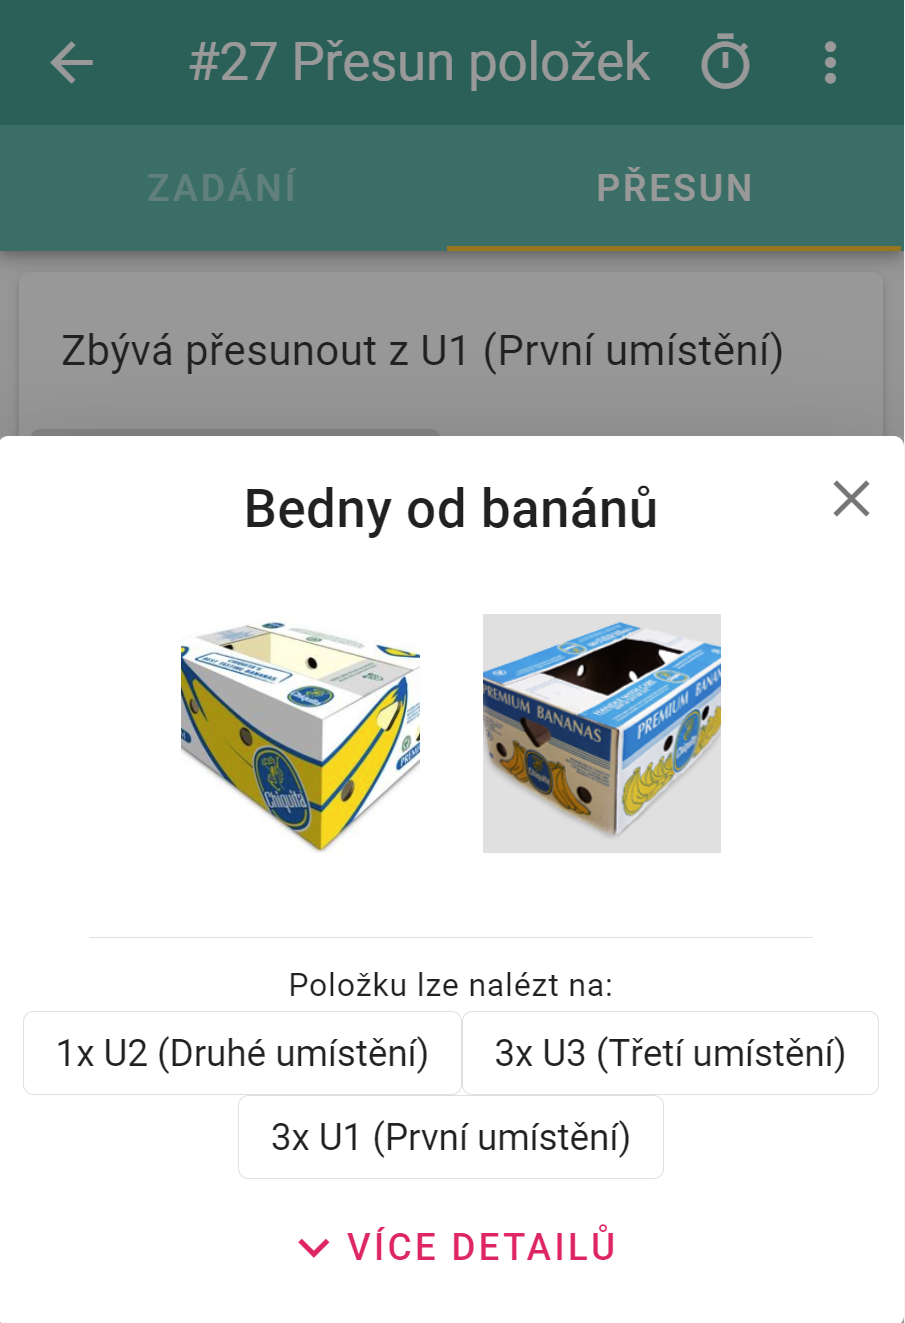
\includegraphics[width=0.6\textwidth]{../png/app_testing/close_bottom_sheet.png}}
\caption[Zavření přehledu skladové položky]{Zavření přehledu skladové položky: křížek v pravém horním rohu byl přidán po uživatelském testování.} \label{picture:test:close_bottom_sheet}
\end{figure}
